% !TeX root = ../main.tex

\appendix{D}{Complete Group-Time ATT Dynamics }
\label{complete_group_time_att_dynamics}
Applying \cite{callaway2021difference}'s approach involves estimating the ATT for each treatment-timing group and calender month. Then, a family of causal parameters of interest can be obtained, which can be aggregated through Equation \ref{eq:event_aggregation} to recover the event study. In the main text, we present the event-study-like results, which are based on the aggregated ATT by the number of months after the treatment. One might wonder if there are heterogeneous treatment effects across different treatment-timing groups so we include the complete group-time ATT here for futher discussions.

Through the following set of figures, we can generally claim that there is no substantial heterogeneous treatment effects across different treatment-timing groups as there is no particular group exhibit distinct ATT dynamics compared to the others in any of the outcome. However, theris a exception, which is ATT of residential shift on outgoing contact distance in group 7 (see Figure \ref{fig:attgt_residential_shift_mobile_communication_network}). In such case, only group 7 shows a significant positive effect contemporaneously with the treatment while all the other groups exhibit insignificant effects. However, all the others are, in fact, experience a positive upward shift in outcomes, which coincides with the group 7 and therefore, we can still somehow confirm the positive effect of residential shift on outgoing contact distance.

\clearpage\newpage
\begin{figure}[ht!]
\centering
\caption{The Effects of Residential Shift on Mobile Communication Network Features}


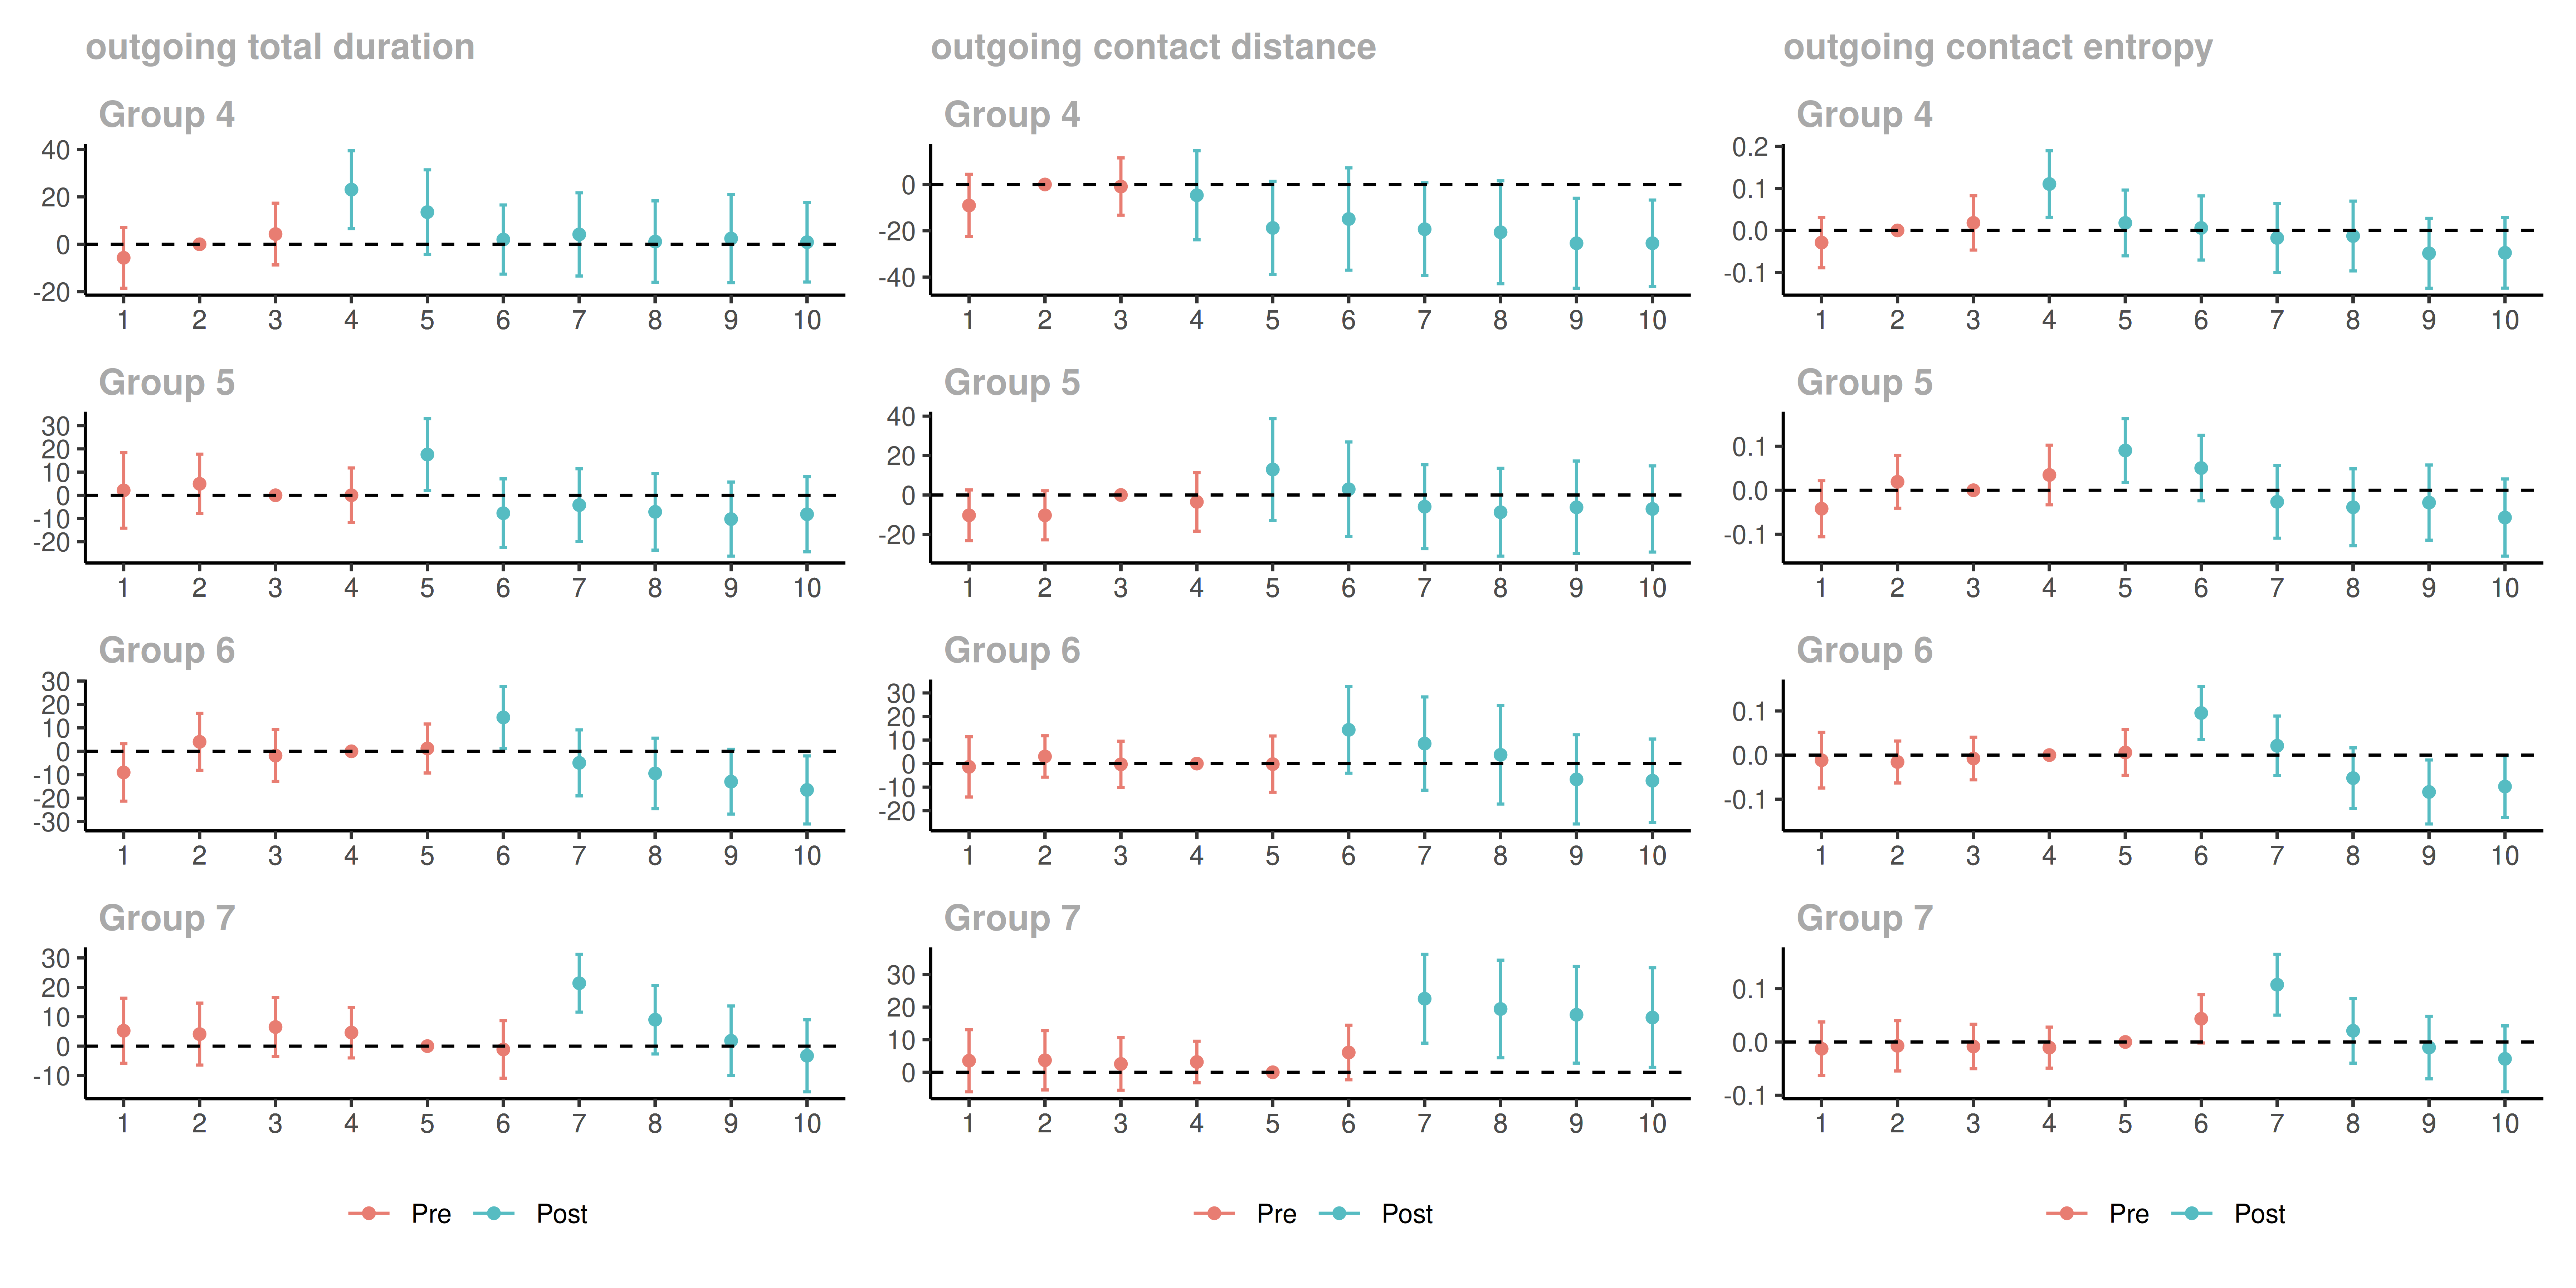
\includegraphics[width=1.5\textwidth, angle=90]{figures/csdid/cohort_specific_ATT_dynamics/residential_shift_mobile_communication_network.png}

% \caption*{Notes: }
\label{fig:attgt_residential_shift_mobile_communication_network}
\end{figure}


\clearpage\newpage
\begin{figure}[ht!]
\centering
\caption{The Effects of Residential Shift on Mobility Features}


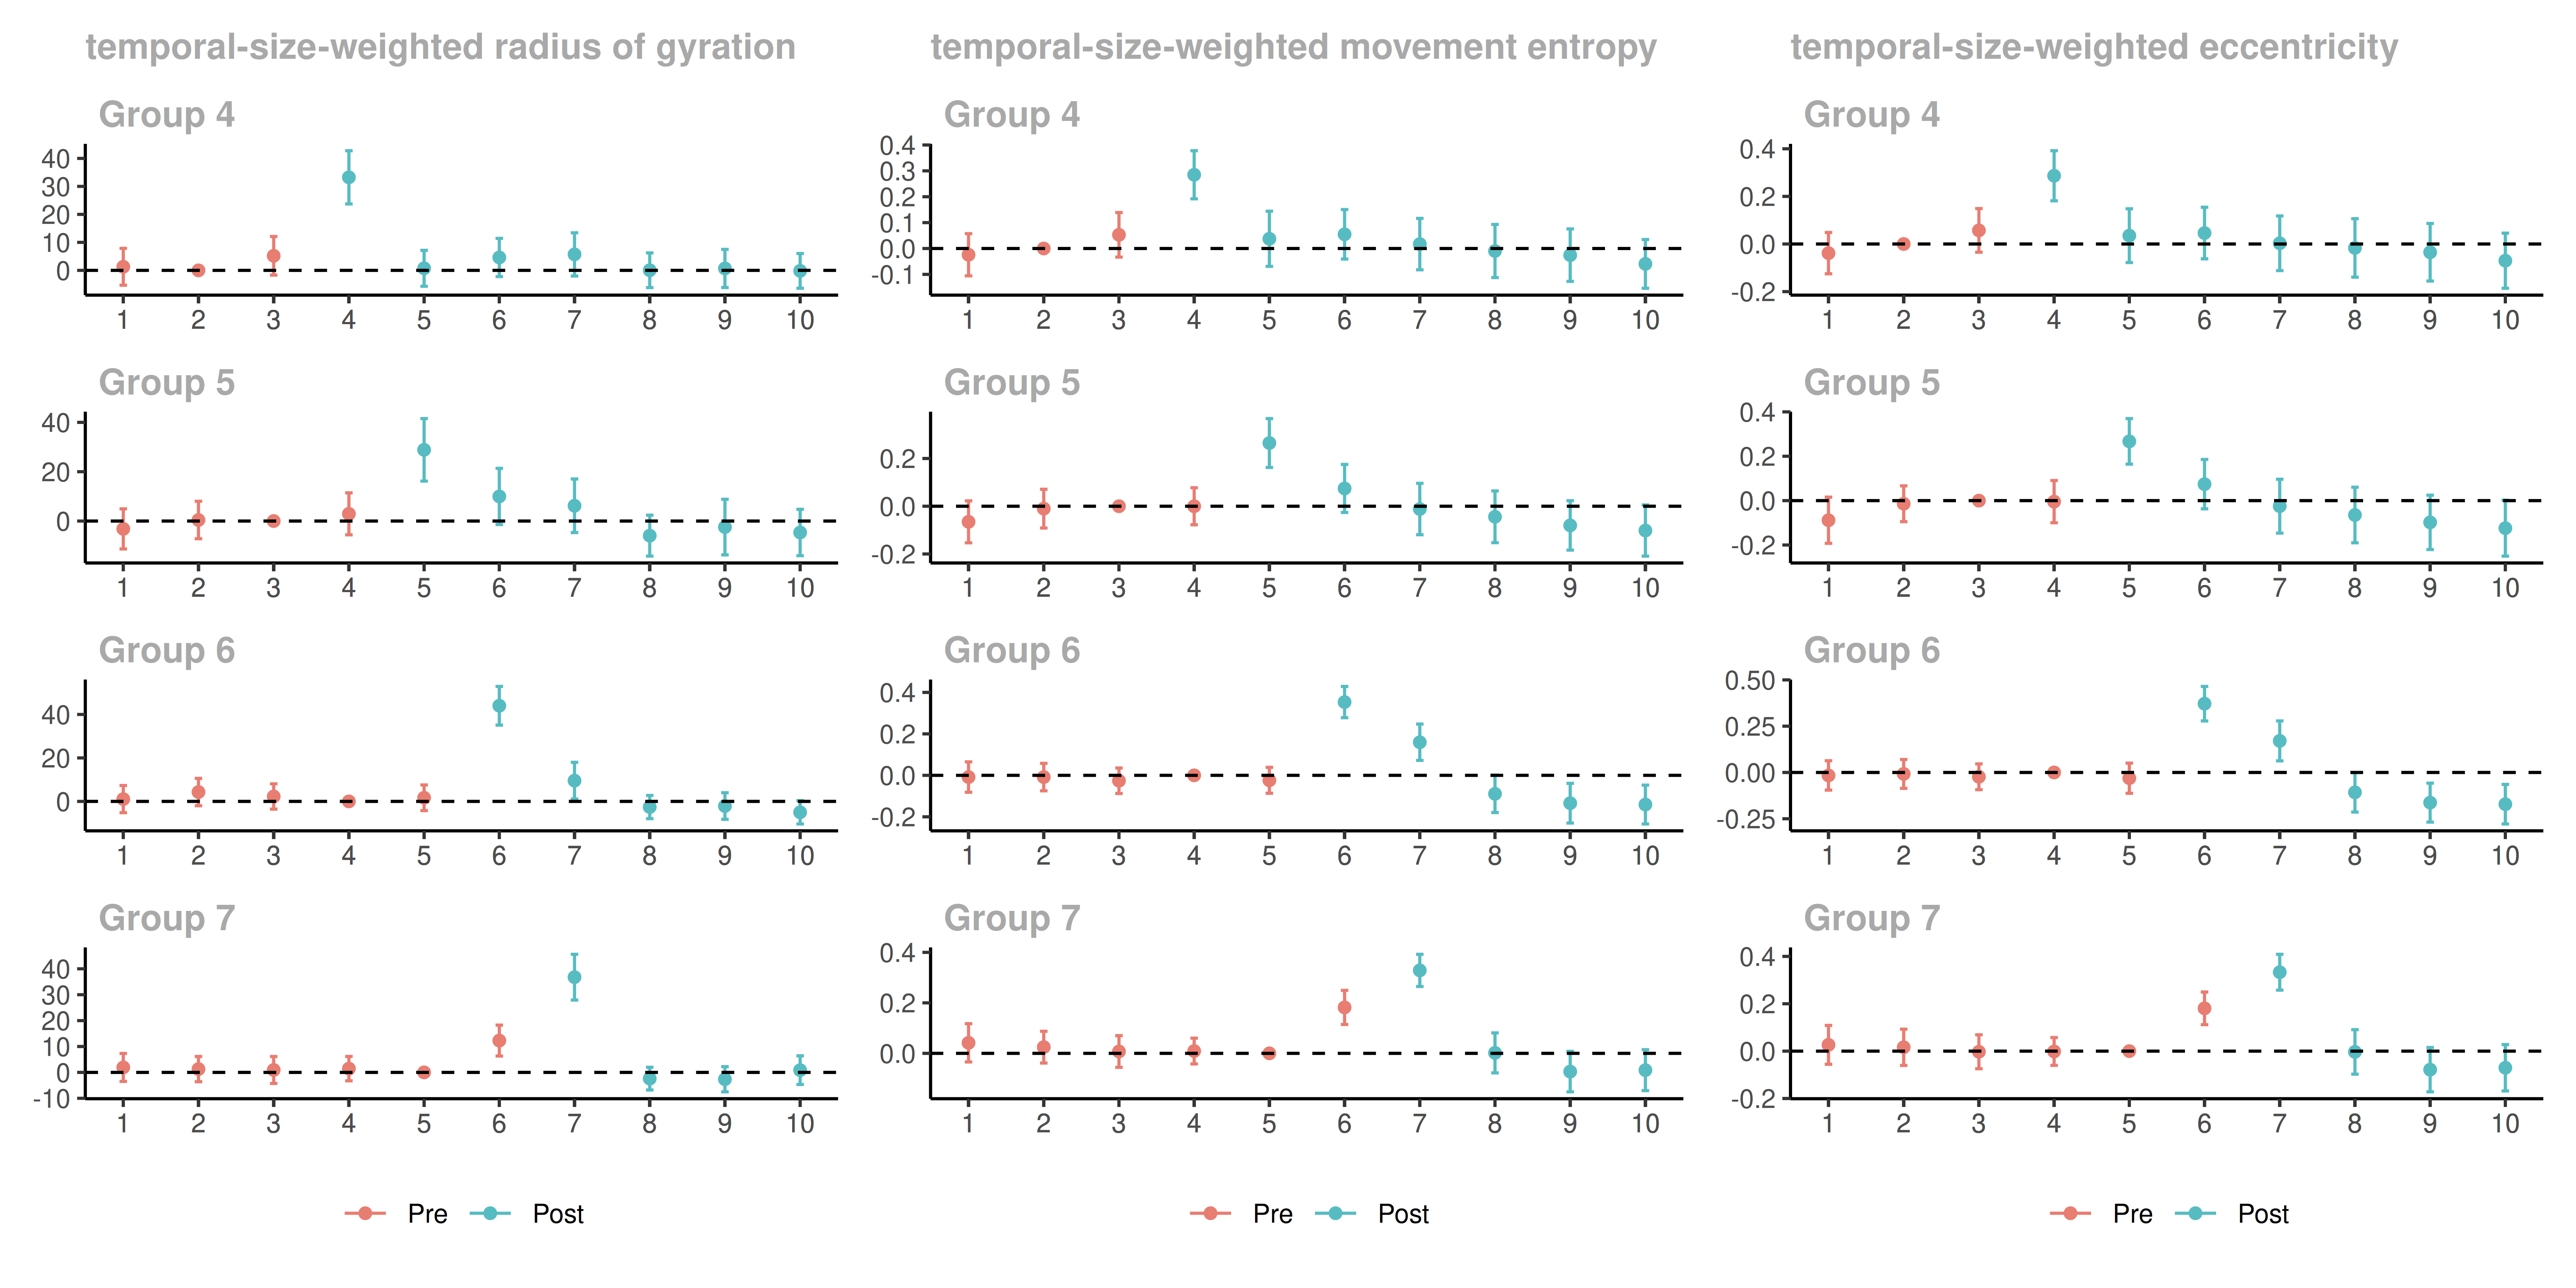
\includegraphics[width=1.5\textwidth, angle=90]{figures/csdid/cohort_specific_ATT_dynamics/residential_shift_mobility.png}

% \caption*{Notes:}
\label{fig:attgt_residential_shift_mobility}
\end{figure}


\clearpage\newpage
\begin{figure}[ht!]
\centering
\caption{The Effects of Smartphone Adoption on Mobile Communication Network Features}


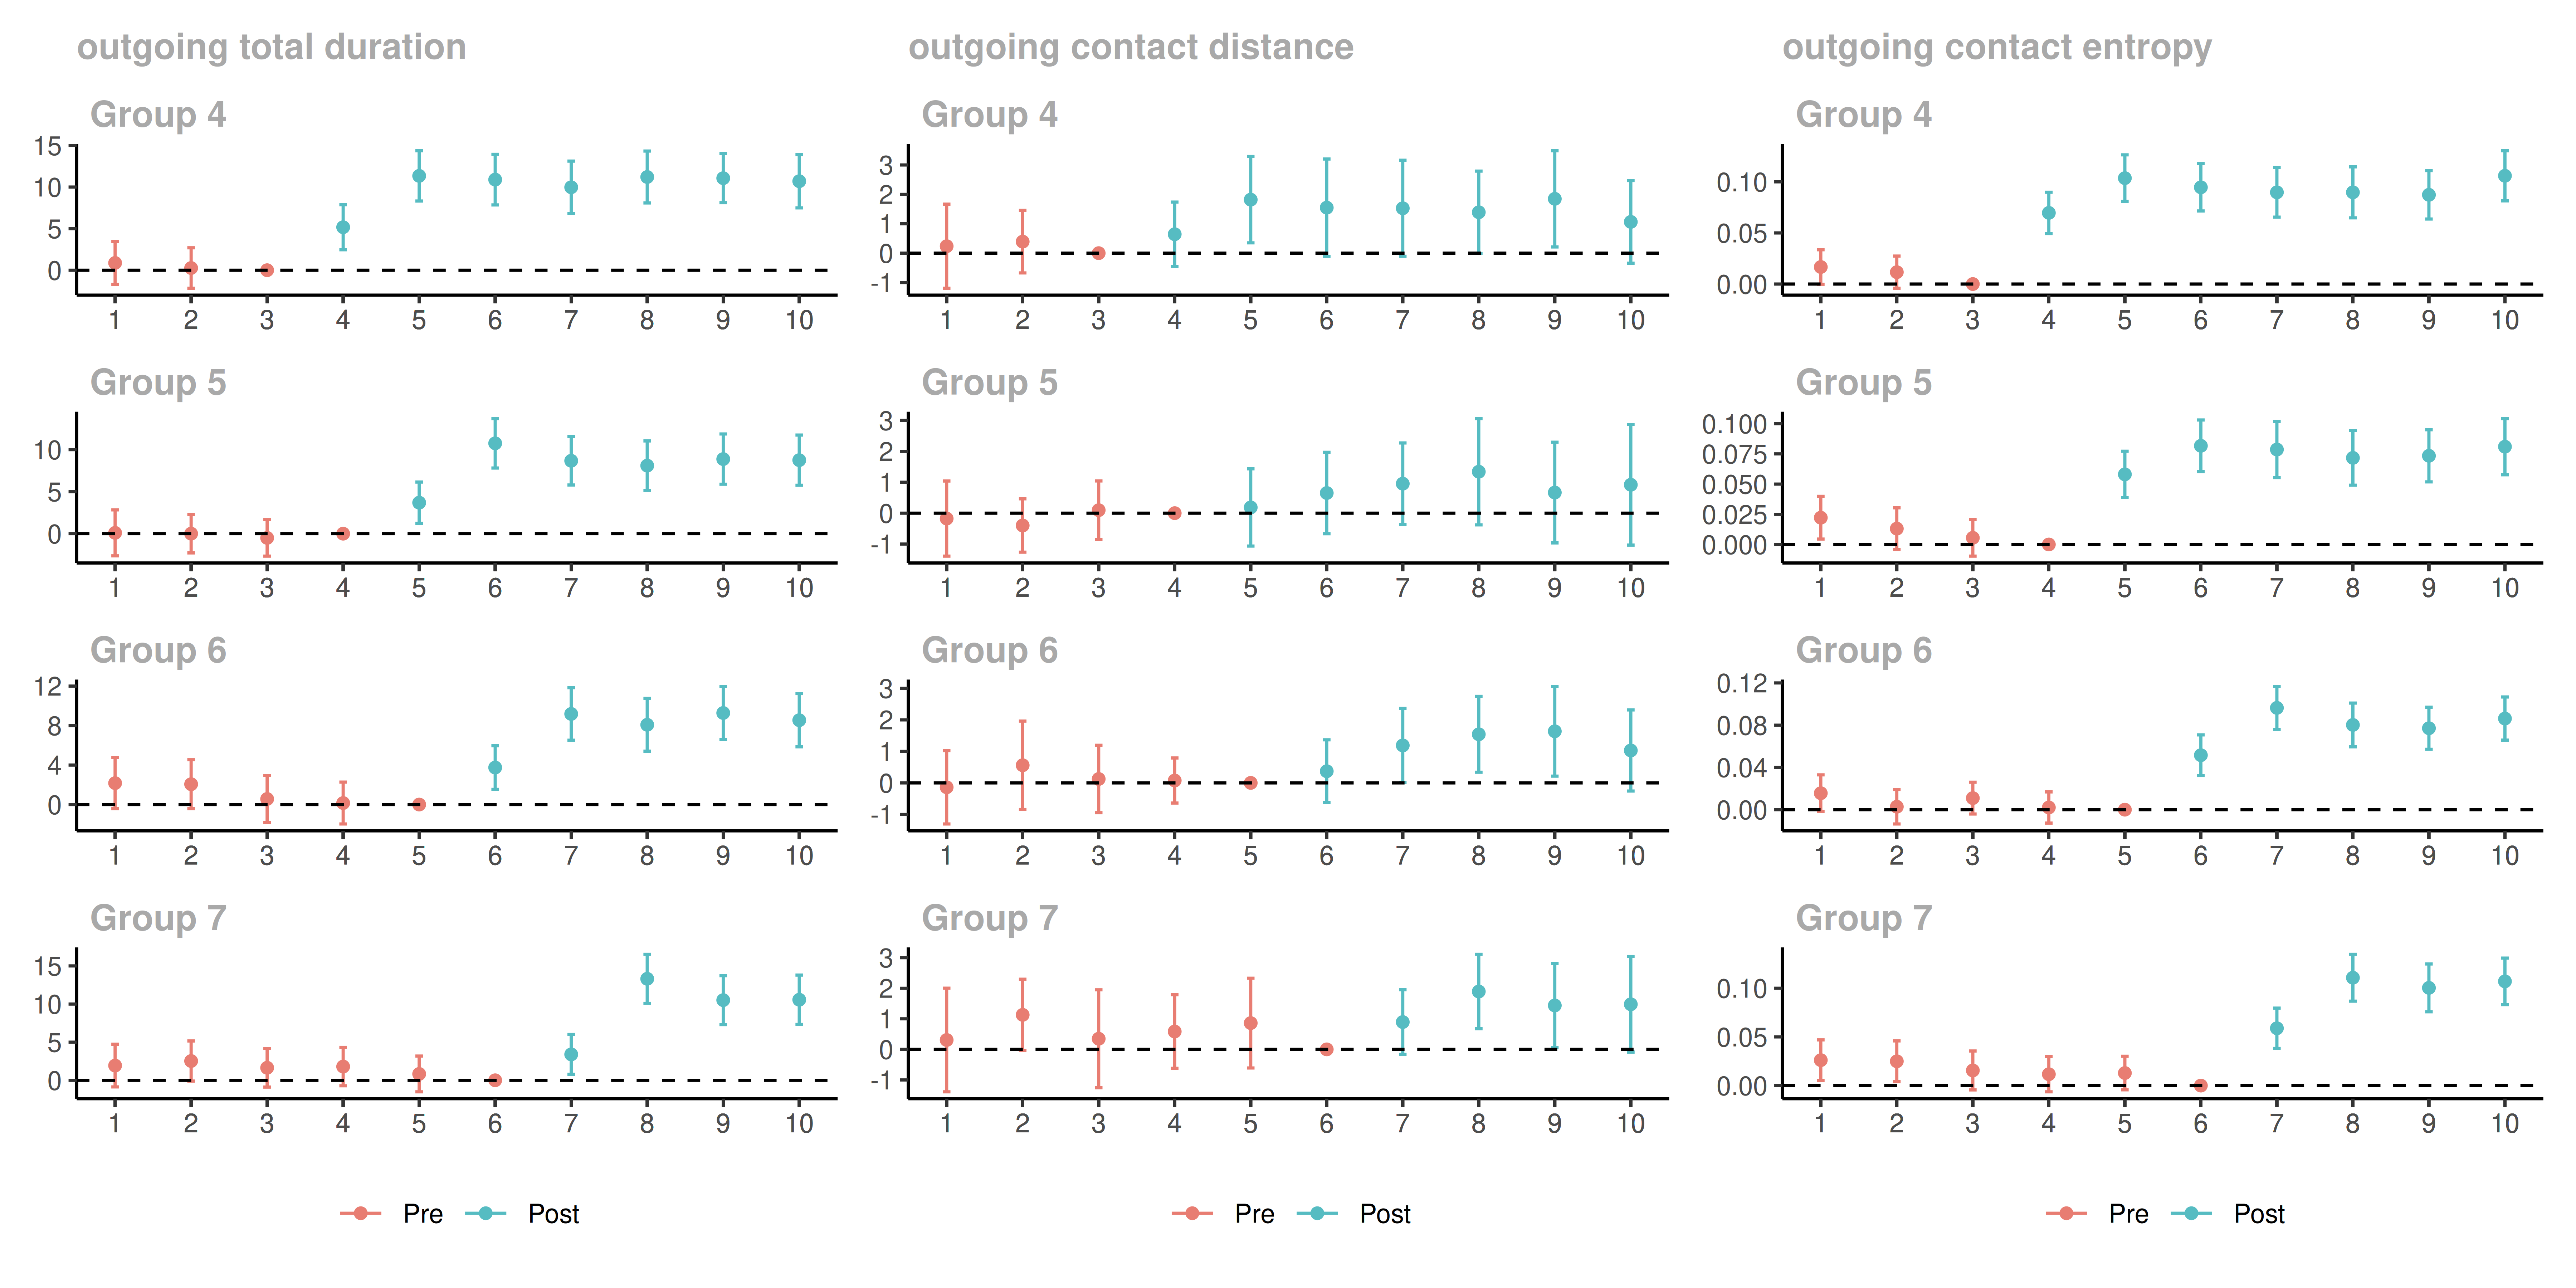
\includegraphics[width=1.5\textwidth, angle=90]{figures/csdid/cohort_specific_ATT_dynamics/smartphone_adoption_mobile_communication_network.png}

% \caption*{Notes:}
\label{fig:attgt_smartphone_adoption_mobile_communication_network}
\end{figure}


\clearpage\newpage
\begin{figure}[ht!]
\centering
\caption{The Effects of Smartphone Adoption on Mobility Features}

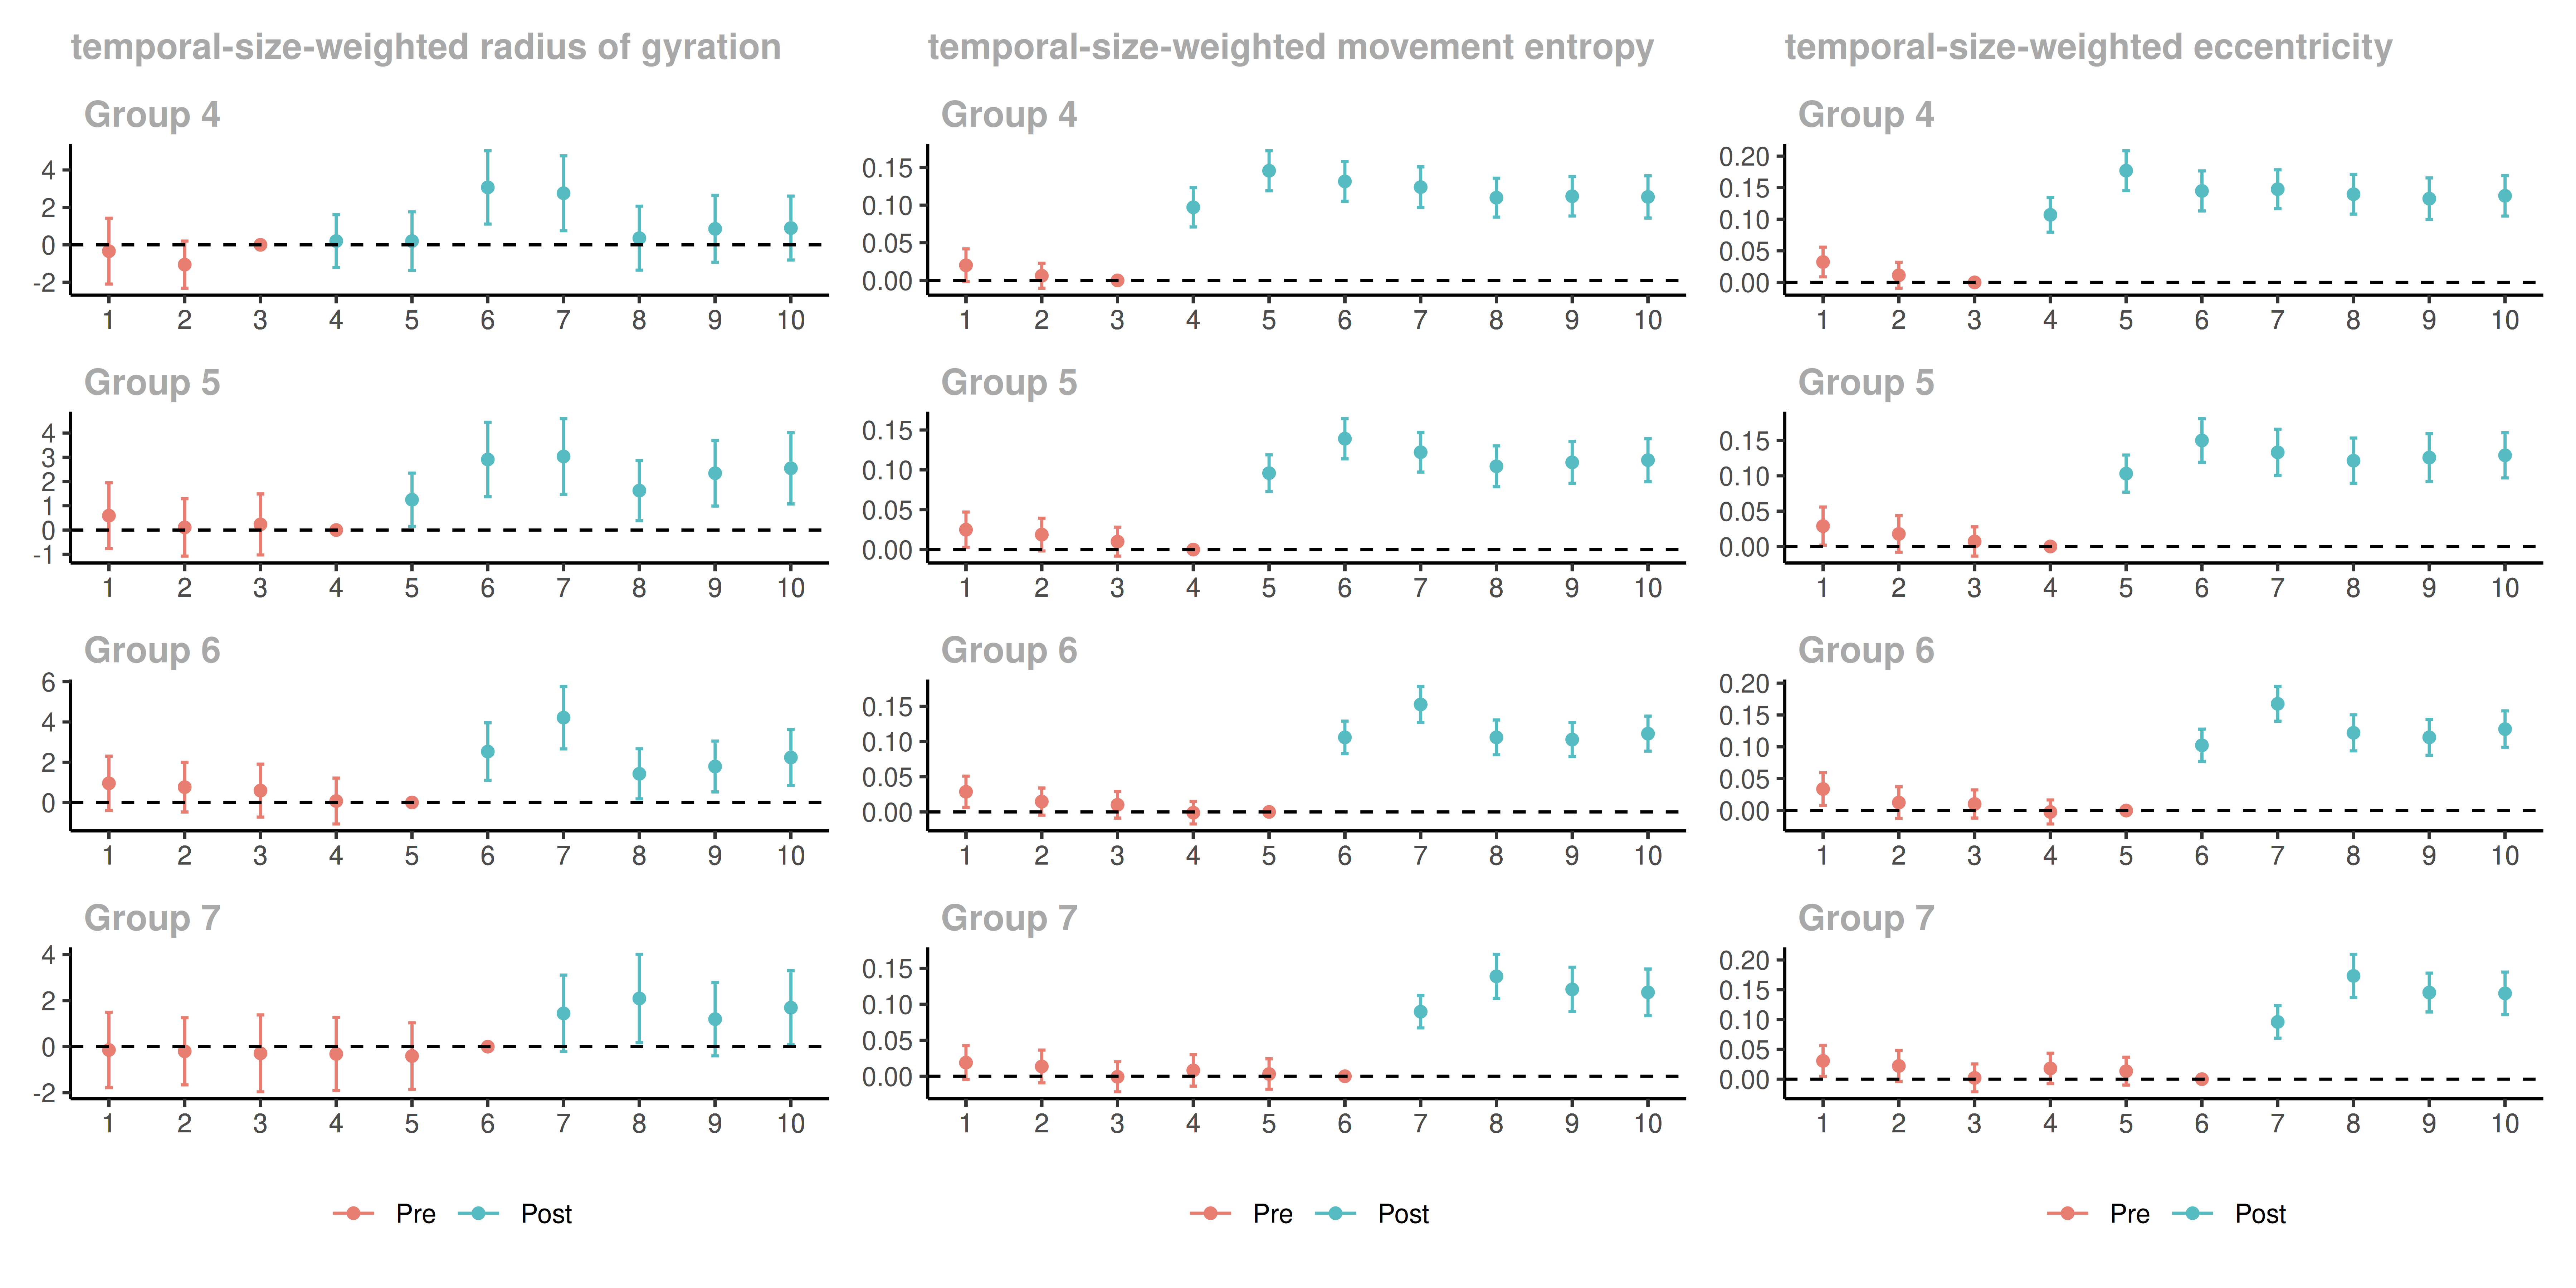
\includegraphics[width=1.5\textwidth, angle=90]{figures/csdid/cohort_specific_ATT_dynamics/smartphone_adoption_mobility.png}

% \caption*{Notes:}
\label{fig:attgt_smartphone_adoption_mobility}
\end{figure}
